\chapter{Background}
\label{background}

\section{Introduction to Machine Learning}
In \textcite{MLANN}, Machine Learning is defined as "the question of how to
construct computer programs that automatically improve with experience".
Machine Learning has blossomed in recent years with applications across multiple
domains using vastly different paradigms and technologies.

There are many ways in which Machine Learning can be used in the modern world,
many of which are being utilised to great affect.
Some of these applications, are image recognition, natural language processing,
medical diagnosis and many more.
There may be fear that Machine Learning will start to take away many jobs from
humans but this may not be the case. Imagine a doctor, having to diagnose a
patient, a machine can offer suggestions based on very large datasets of what
the diagnosis is. This is not to say that a Machine would be
perscribing patients, but merely act as an assistant to the doctor.

Machine Ethics is a large problem that comes hand in hand with Machine Learning.
There is a very important question of who takes the blame when things go wrong,
that is why I think it is important that we only use Machine Learning to advise
and not to determine but this can be very difficult in a world where, for
example, an autonomous car has to decide between crashing into a vehicle beside
them with an unknown number of people inside or the two children playing in the
street.

One of the most exciting avenues in Machine Learning, in my opinion, is Computer
Vision. Computer Vision can be used in many areas to improve our lives. As
mentioned earlier, autonomous cars are only possible when a machine can
determine what objects are around it. Computer Vision can allow a machine to
recognise skin diseases in an image. The applications are nearly limitless and
that is without taking into account other uses.

\section{Machine Learning Paradigms}
There are many Machine Learning paradigms, all of which I will
discuss briefly below, but the main area of my focus for this project is in
Artificial Neural Networks (ANN). This is because I have researched extensively into Convolutional Neural Networks which are based on ANN's.
\subsection{Artificial Neural Networks}
An Artificial Neural Network is a bio-inspired system that is used to model the human brain in how it learns from experience.
The ANN uses this model to build a very complex web of connected units called
artificial neurons.
These nuerons are connected by certain weights which determines the processing
capacity of the network and these weights are created by learning a
dataset.(Malachy)
An ANN has a set of inputs that take in a value, sometimes from network outputs
and produce a single result or classification.
While an ANN is bio-inspired from the human brain, there are many elements of
the brain that are not present in ANN and many new elements in ANN that are not
modelled from the human brain.

Before I can talk about Convolution Neural Networks which are vital the image
processing, I will have to talk about the perceptron learning algorithm, the multi
layer percepton, and backpropogation.

\subsubsection{Perceptron Learning - Artificial Neuron}
In our Artificial Neural Network a Perecptron is an Artificial Neuron.
It is called an Artifical Neuron because it is a bio-inspired neuron which models
a neuron in the human brain in terms of inputs and output.

In Perceptron learning, we can take two inputs which are put towards an
activation function with a bias attached as seen in \ref{fig:perceptron}.
These inputs are multiplied by the weights that connect the input to the
activation function and depending on the result, the activation function may
fire an output.

\begin{figure}
     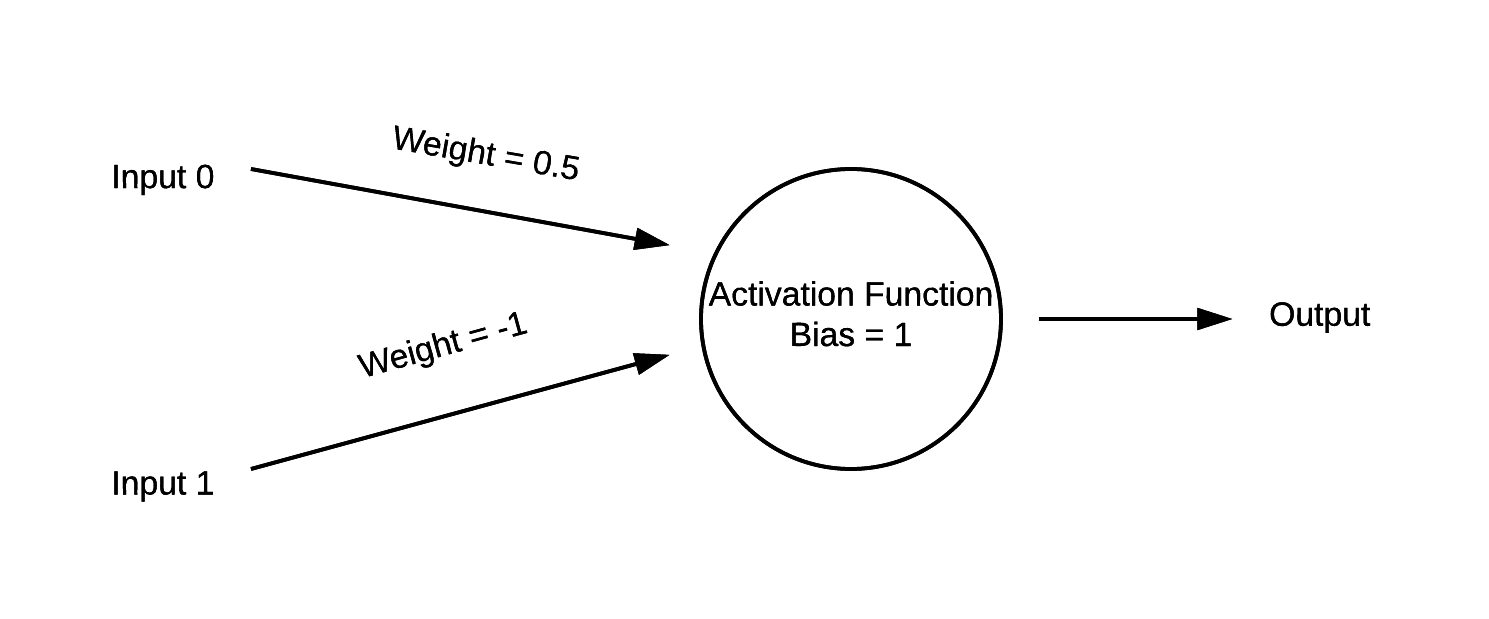
\includegraphics{Perceptron}
     \caption{Perceptron}
     \label{fig:perceptron}
\end{figure}

This Perceptron Learning Rule assumes that there are two sets of instances, a
positive and negative set, and each of these has an input and output domain.

\subsubsection{Multi Layered Perceptron}
Multi Layer Perceptrons (MLP) are made up of multiple layers of perceprons connected
together.
Firstly, we have an input layer, followed by one of more hidden layers and then
finally an output layer.
Any Neural Network with more than three hidden layers is categorised as a deep
layer.

Multi Layer Perceptrons are a class of feed forward Artificial Neural Networks.
These means that the output of each perceptron feeds into an input in the next
layer of the network.

\begin{figure}
    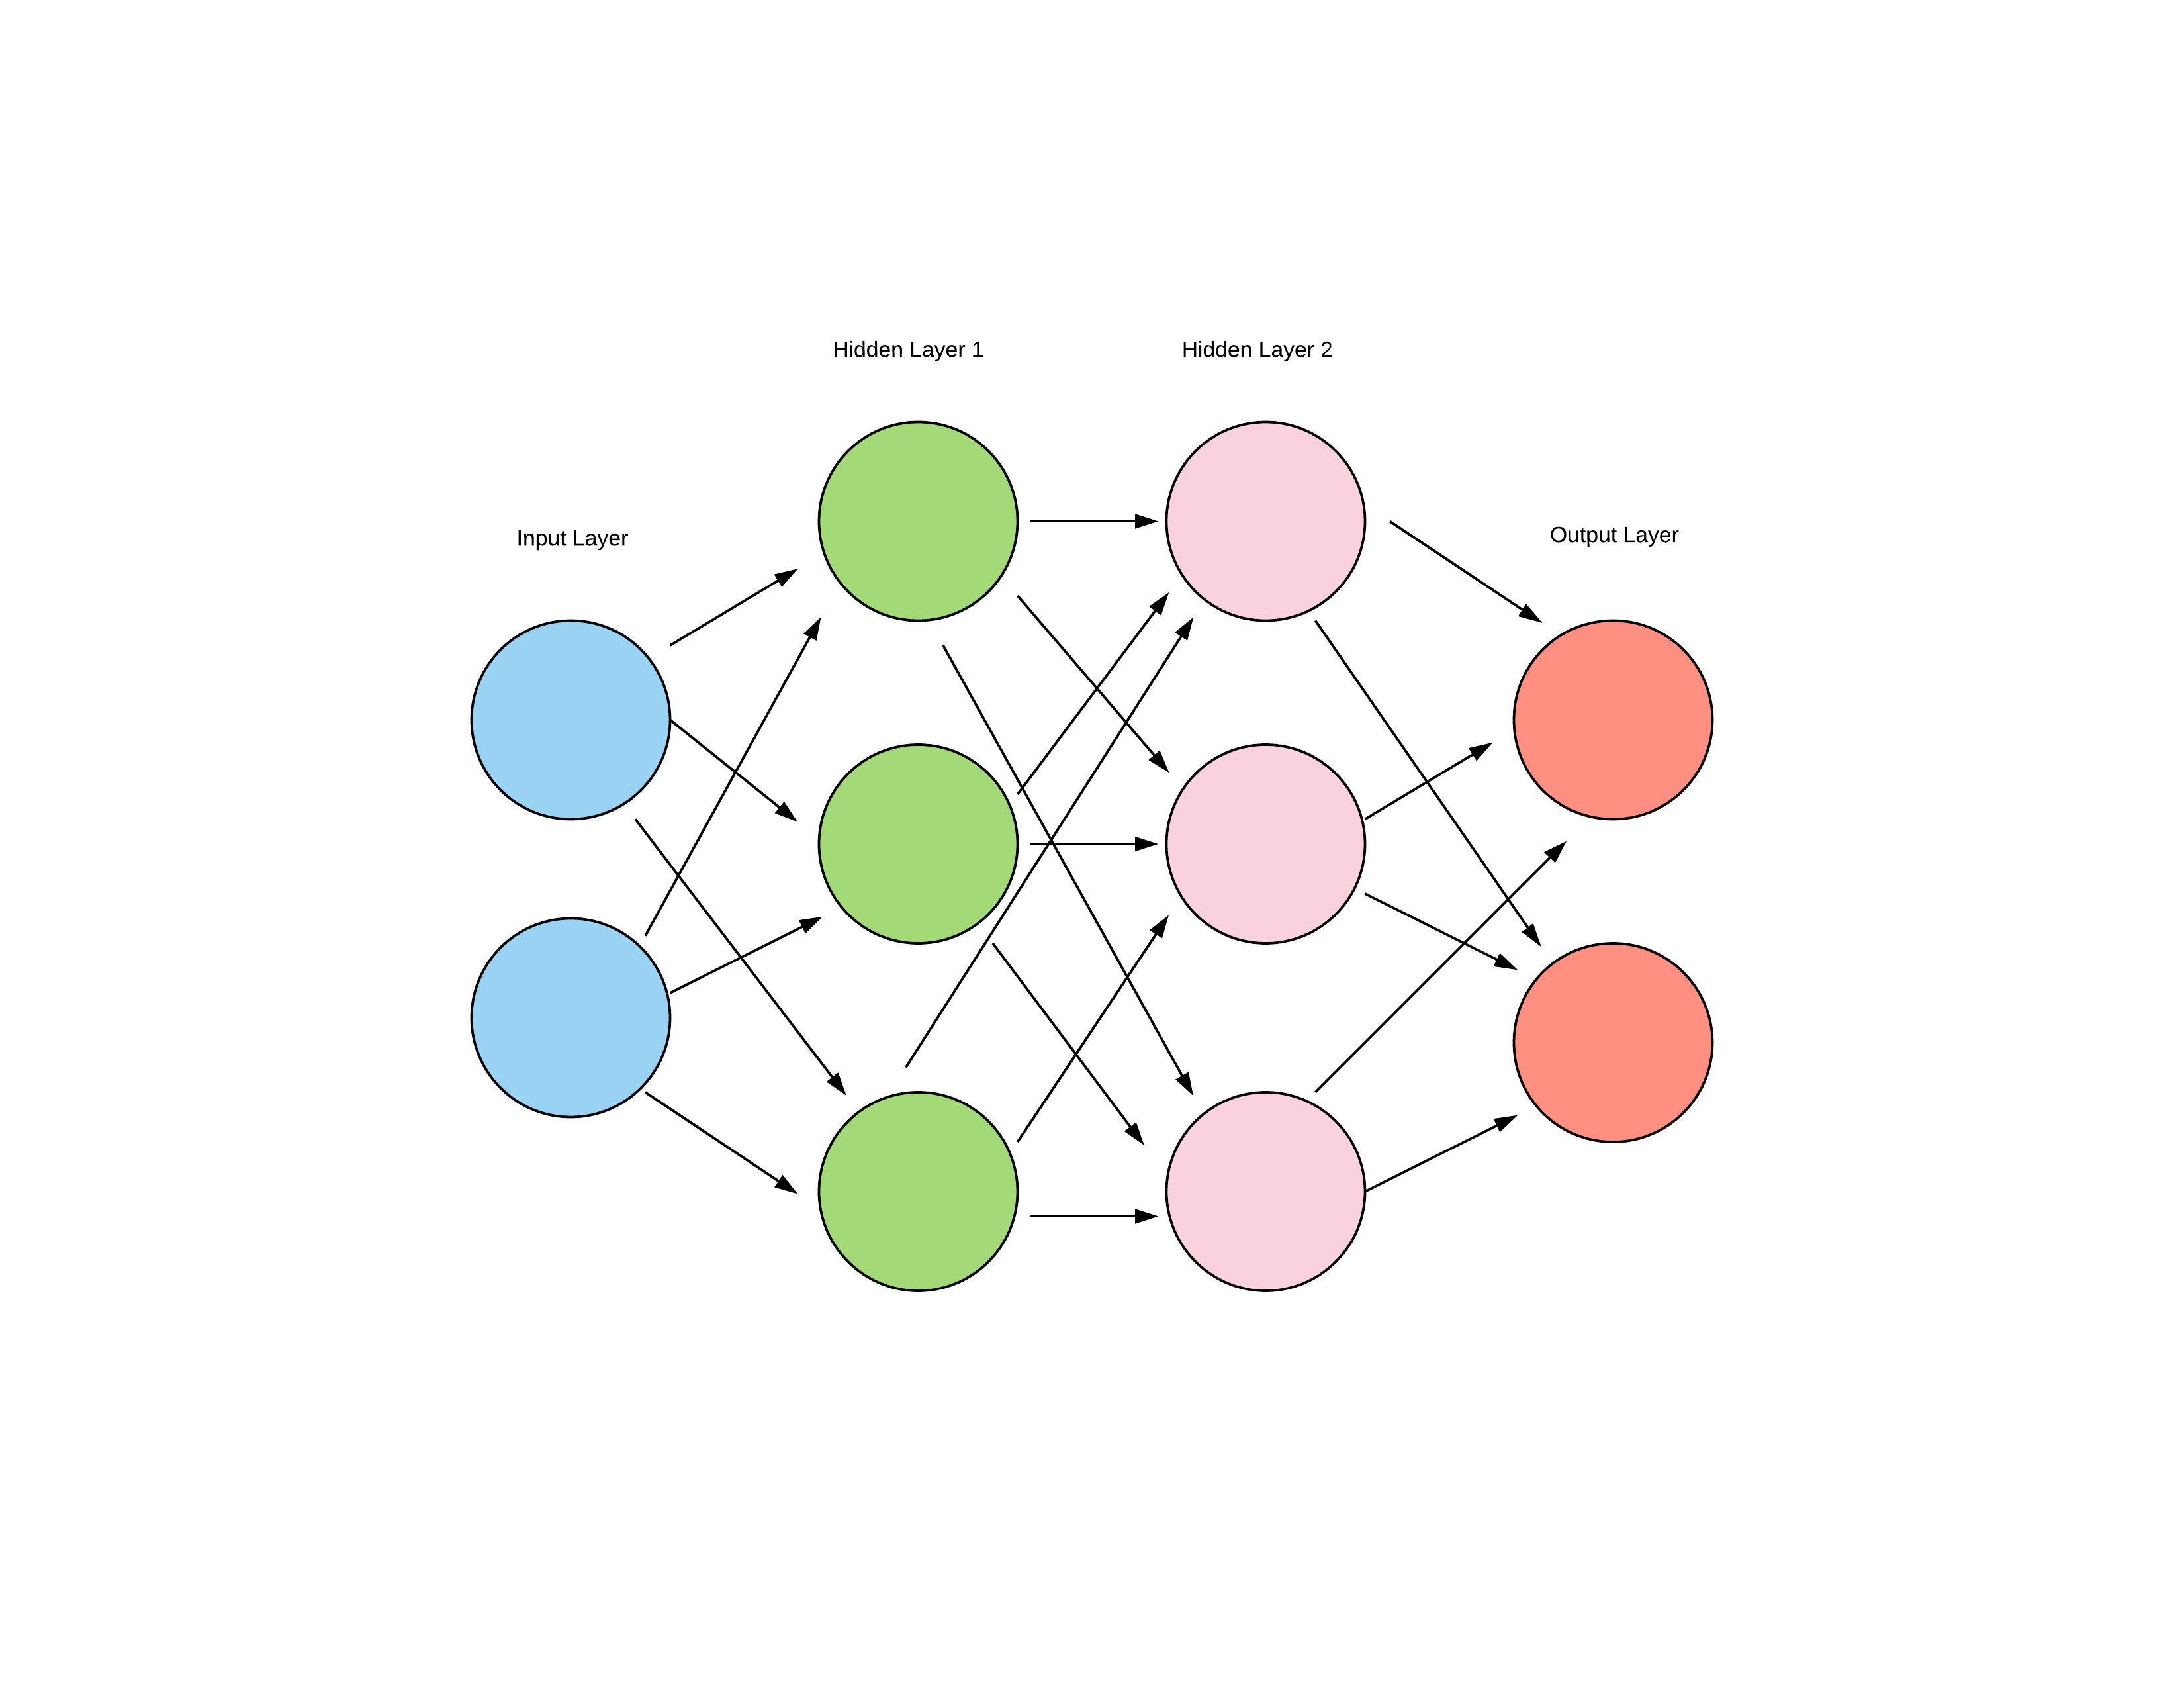
\includegraphics[width=150mm,scale=0.5]{mlp}
     \caption{Multi Layer Perceptron}
     \label{fig:mlp}
\end{figure}

\subsubsection{Gradient Descent and Backpropogation}

\subsubsection{Convolutional Neural Networks}
Convolutional Neural Networks (CNN's) are essentially a Multi Layered Percetron with a
special structure. CNN's have one major difference from a MLP, they have extra
layer of convolution and pooling.

Figure \ref{fig:XtoRec} show an image that we want to compare against
Figure \ref{fig:XtoComp}.
For humans, it is quite easy to determine that these images are very similar but
for a computer this task is surprisingly difficult.

So what a CNN does, to combat this problem, is to take a small feature from
Figure \ref{fig:XtoRec} and compare it to a subsection of Figure \ref{fig:XtoComp}.
The CNN multiplies the feature and a section of Figure \ref{fig:XtoComp}, adds
up the results and divides by 9. This then gives a decimal value of how likely
it is that the feature is in the part of the image, as seen in Figure
\ref{fig:convoluted}.
This is called filtering. The Convolutional layer is composed of carrying out
this filtering for every single possible location in Figure \ref{fig:XtoComp}.
\begin{figure}
      \begin{subfigure}[b]{0.4\textwidth}
          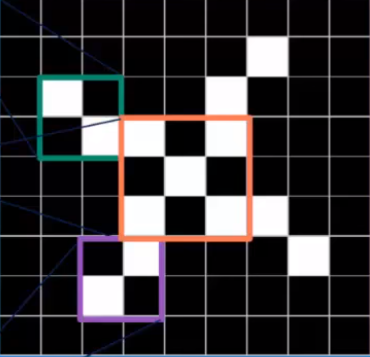
\includegraphics[width=\textwidth]{XtoRec}
          \caption{Image to Classify}
          \label{XtoRec}
      \end{subfigure}
    %
      \begin{subfigure}[b]{0.4\textwidth}
      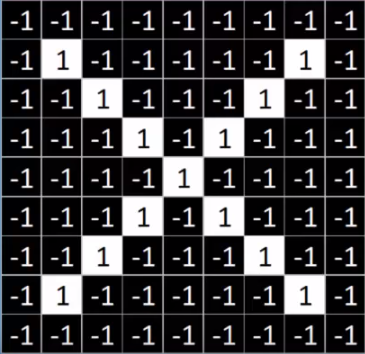
\includegraphics[width=\textwidth]{XtoComp}
      \caption{Image to Compare}
      \label{XtoComp}
      \end{subfigure}
\end{figure}

\begin{figure}
      \begin{subfigure}[b]{0.4\textwidth}
          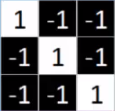
\includegraphics[width=\textwidth]{ImageFeature}
          \caption{Image Feature to Search}
          \label{fig:feature}
      \end{subfigure}
     %
      \begin{subfigure}[b]{0.4\textwidth}
           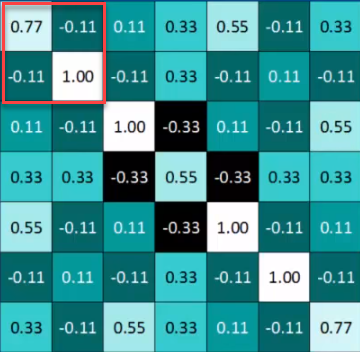
\includegraphics[width=\textwidth]{ConvImage}
           \caption{Convoluted Image}
           \label{fig:convoluted}
      \end{subfigure}
\end{figure}
\begin{figure}
    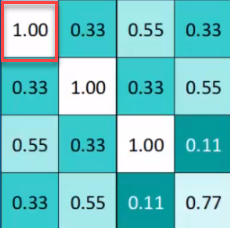
\includegraphics[width=50mm,scale=0.5]{PooledImage}
    \caption{Pooled Image}
    \label{fig:pooled}
\end{figure}
Next is the Pooling Layer, what this layer does, is it takes the convoluted
layer output, you can use Figure \ref{fig:convoluted} as reference, and from a
user defined size ie. 2x2, gets either the highest decimal value (Max pooling)
or the average value (Mean pooling) and records that as the new value for the
section. This is then applied to the entire image. As we can see in Figure
\ref{fig:pooled} we know have a much smaller image stack in which to classify,
thus making the computation easier.

In between the Convolution and Pooling layer, there is sometimes a Normalization
layer. This Normalization layer creates Rectified Linear Units (RLU's). In other
words, if we take Figure \ref{fig:convoluted}, it changes all minus values to
zero.

\subsubsection{Fully Convolutional Networks}
A Fully Convolutional Network is one that does not have a fully connected layer
and in a fully connected layers place is another convolution layer.

\subsection{Other Paradigms}
There are many other Machine Learning paradigms, of which I will give a brief
introduction.

\subsubsection{Decision Trees}
"Decision tree learning is  method for approcimating disrete-valued target
functions, in which the learned function is represented by a descision tree"
\textcite{MLDT}.

\subsubsection{Meta/Ensemble Classifiers}
\subsubsection{Logistic Regression}
\subsubsection{Support Vector Machine}
\subsubsection{Regression Analysis}
\subsubsection{Unsupervised Learning}
\subsubsection{Reinforcement Learning}

\section{Overview of Machine Vision Approaches to Identification and Classification}
\subsection{Identification}
\subsection{Classification}

\section{API's}

\section{Evaluating the Output}


